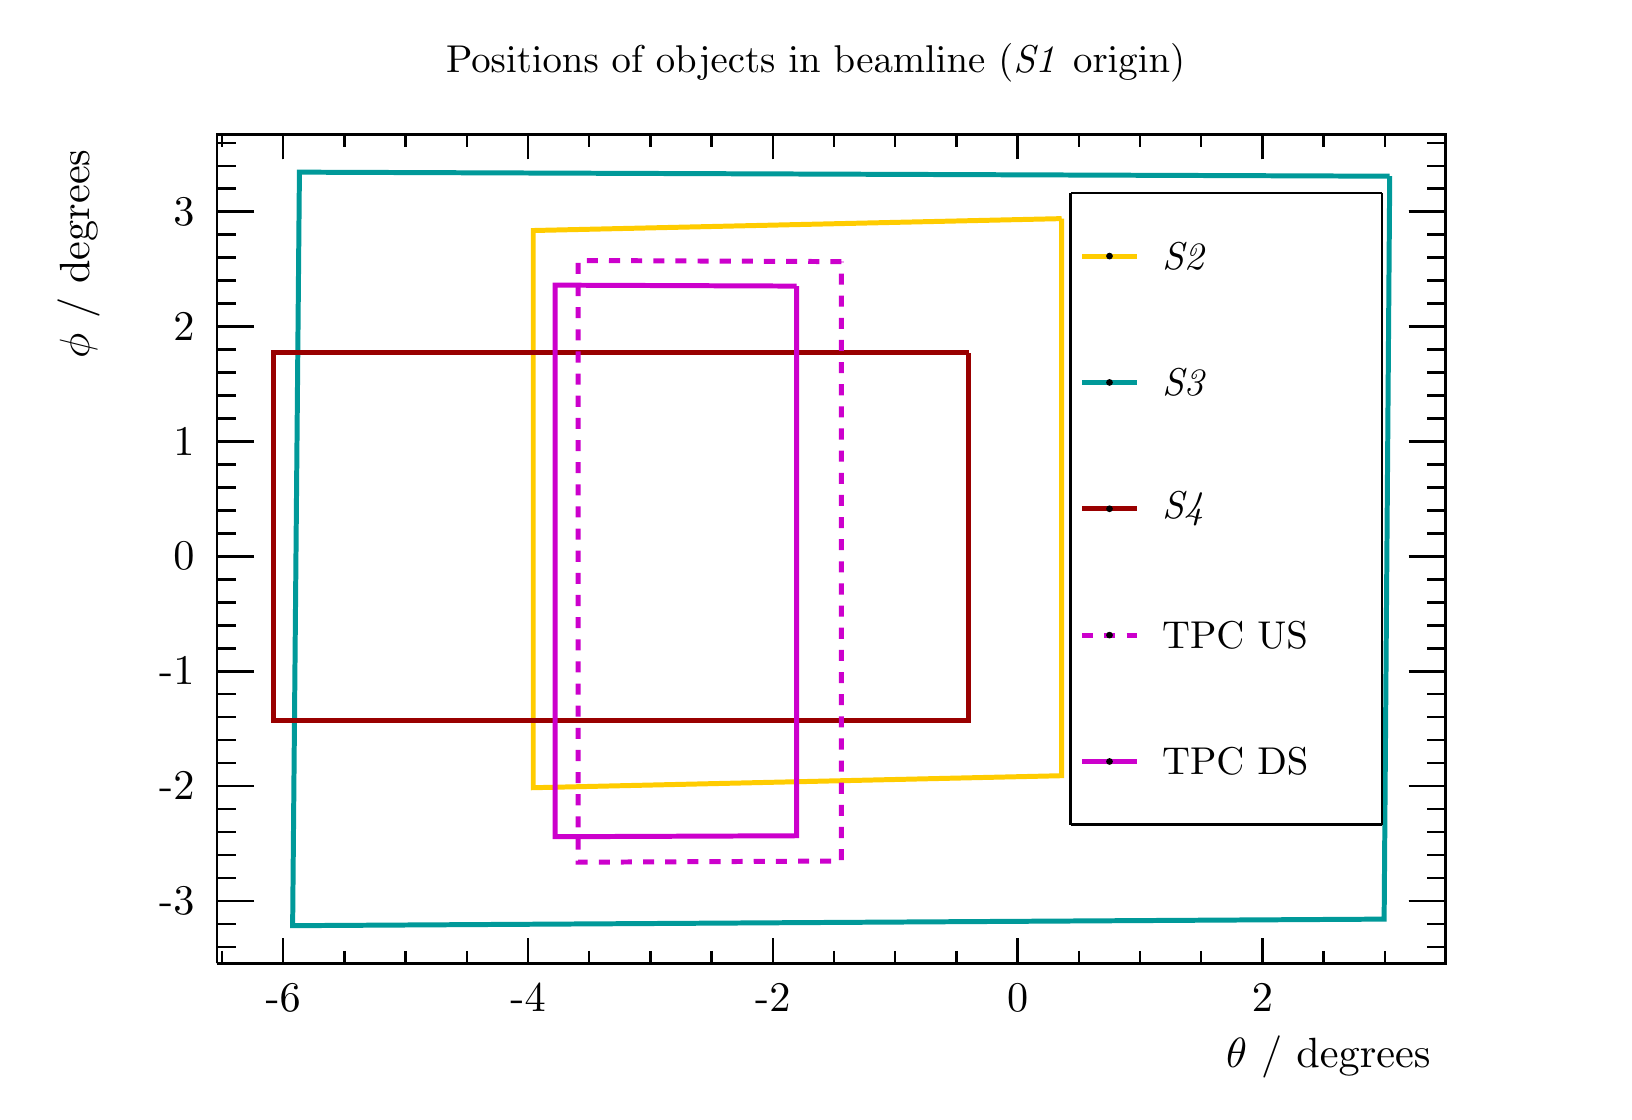
\begin{tikzpicture}
\pgfdeclareplotmark{cross} {
\pgfpathmoveto{\pgfpoint{-0.3\pgfplotmarksize}{\pgfplotmarksize}}
\pgfpathlineto{\pgfpoint{+0.3\pgfplotmarksize}{\pgfplotmarksize}}
\pgfpathlineto{\pgfpoint{+0.3\pgfplotmarksize}{0.3\pgfplotmarksize}}
\pgfpathlineto{\pgfpoint{+1\pgfplotmarksize}{0.3\pgfplotmarksize}}
\pgfpathlineto{\pgfpoint{+1\pgfplotmarksize}{-0.3\pgfplotmarksize}}
\pgfpathlineto{\pgfpoint{+0.3\pgfplotmarksize}{-0.3\pgfplotmarksize}}
\pgfpathlineto{\pgfpoint{+0.3\pgfplotmarksize}{-1.\pgfplotmarksize}}
\pgfpathlineto{\pgfpoint{-0.3\pgfplotmarksize}{-1.\pgfplotmarksize}}
\pgfpathlineto{\pgfpoint{-0.3\pgfplotmarksize}{-0.3\pgfplotmarksize}}
\pgfpathlineto{\pgfpoint{-1.\pgfplotmarksize}{-0.3\pgfplotmarksize}}
\pgfpathlineto{\pgfpoint{-1.\pgfplotmarksize}{0.3\pgfplotmarksize}}
\pgfpathlineto{\pgfpoint{-0.3\pgfplotmarksize}{0.3\pgfplotmarksize}}
\pgfpathclose
\pgfusepathqstroke
}
\pgfdeclareplotmark{cross*} {
\pgfpathmoveto{\pgfpoint{-0.3\pgfplotmarksize}{\pgfplotmarksize}}
\pgfpathlineto{\pgfpoint{+0.3\pgfplotmarksize}{\pgfplotmarksize}}
\pgfpathlineto{\pgfpoint{+0.3\pgfplotmarksize}{0.3\pgfplotmarksize}}
\pgfpathlineto{\pgfpoint{+1\pgfplotmarksize}{0.3\pgfplotmarksize}}
\pgfpathlineto{\pgfpoint{+1\pgfplotmarksize}{-0.3\pgfplotmarksize}}
\pgfpathlineto{\pgfpoint{+0.3\pgfplotmarksize}{-0.3\pgfplotmarksize}}
\pgfpathlineto{\pgfpoint{+0.3\pgfplotmarksize}{-1.\pgfplotmarksize}}
\pgfpathlineto{\pgfpoint{-0.3\pgfplotmarksize}{-1.\pgfplotmarksize}}
\pgfpathlineto{\pgfpoint{-0.3\pgfplotmarksize}{-0.3\pgfplotmarksize}}
\pgfpathlineto{\pgfpoint{-1.\pgfplotmarksize}{-0.3\pgfplotmarksize}}
\pgfpathlineto{\pgfpoint{-1.\pgfplotmarksize}{0.3\pgfplotmarksize}}
\pgfpathlineto{\pgfpoint{-0.3\pgfplotmarksize}{0.3\pgfplotmarksize}}
\pgfpathclose
\pgfusepathqfillstroke
}
\pgfdeclareplotmark{newstar} {
\pgfpathmoveto{\pgfqpoint{0pt}{\pgfplotmarksize}}
\pgfpathlineto{\pgfqpointpolar{44}{0.5\pgfplotmarksize}}
\pgfpathlineto{\pgfqpointpolar{18}{\pgfplotmarksize}}
\pgfpathlineto{\pgfqpointpolar{-20}{0.5\pgfplotmarksize}}
\pgfpathlineto{\pgfqpointpolar{-54}{\pgfplotmarksize}}
\pgfpathlineto{\pgfqpointpolar{-90}{0.5\pgfplotmarksize}}
\pgfpathlineto{\pgfqpointpolar{234}{\pgfplotmarksize}}
\pgfpathlineto{\pgfqpointpolar{198}{0.5\pgfplotmarksize}}
\pgfpathlineto{\pgfqpointpolar{162}{\pgfplotmarksize}}
\pgfpathlineto{\pgfqpointpolar{134}{0.5\pgfplotmarksize}}
\pgfpathclose
\pgfusepathqstroke
}
\pgfdeclareplotmark{newstar*} {
\pgfpathmoveto{\pgfqpoint{0pt}{\pgfplotmarksize}}
\pgfpathlineto{\pgfqpointpolar{44}{0.5\pgfplotmarksize}}
\pgfpathlineto{\pgfqpointpolar{18}{\pgfplotmarksize}}
\pgfpathlineto{\pgfqpointpolar{-20}{0.5\pgfplotmarksize}}
\pgfpathlineto{\pgfqpointpolar{-54}{\pgfplotmarksize}}
\pgfpathlineto{\pgfqpointpolar{-90}{0.5\pgfplotmarksize}}
\pgfpathlineto{\pgfqpointpolar{234}{\pgfplotmarksize}}
\pgfpathlineto{\pgfqpointpolar{198}{0.5\pgfplotmarksize}}
\pgfpathlineto{\pgfqpointpolar{162}{\pgfplotmarksize}}
\pgfpathlineto{\pgfqpointpolar{134}{0.5\pgfplotmarksize}}
\pgfpathclose
\pgfusepathqfillstroke
}
\definecolor{c}{rgb}{1,1,1};
\draw [color=c, fill=c] (0,0) rectangle (20,13.4957);
\draw [color=c, fill=c] (2.4,1.61948) rectangle (18,12.1461);
\definecolor{c}{rgb}{0,0,0};
\draw [c,line width=0.9] (2.4,1.61948) -- (2.4,12.1461) -- (18,12.1461) -- (18,1.61948) -- (2.4,1.61948);
\definecolor{c}{rgb}{1,1,1};
\draw [color=c, fill=c] (2.4,1.61948) rectangle (18,12.1461);
\definecolor{c}{rgb}{0,0,0};
\draw [c,line width=0.9] (2.4,1.61948) -- (2.4,12.1461) -- (18,12.1461) -- (18,1.61948) -- (2.4,1.61948);
\draw [c,line width=0.9] (2.4,1.61948) -- (18,1.61948);
\draw [c,line width=0.9] (3.23864,1.93528) -- (3.23864,1.61948);
\draw [c,line width=0.9] (4.01586,1.77738) -- (4.01586,1.61948);
\draw [c,line width=0.9] (4.79308,1.77738) -- (4.79308,1.61948);
\draw [c,line width=0.9] (5.5703,1.77738) -- (5.5703,1.61948);
\draw [c,line width=0.9] (6.34753,1.93528) -- (6.34753,1.61948);
\draw [c,line width=0.9] (7.12475,1.77738) -- (7.12475,1.61948);
\draw [c,line width=0.9] (7.90197,1.77738) -- (7.90197,1.61948);
\draw [c,line width=0.9] (8.67919,1.77738) -- (8.67919,1.61948);
\draw [c,line width=0.9] (9.45641,1.93528) -- (9.45641,1.61948);
\draw [c,line width=0.9] (10.2336,1.77738) -- (10.2336,1.61948);
\draw [c,line width=0.9] (11.0109,1.77738) -- (11.0109,1.61948);
\draw [c,line width=0.9] (11.7881,1.77738) -- (11.7881,1.61948);
\draw [c,line width=0.9] (12.5653,1.93528) -- (12.5653,1.61948);
\draw [c,line width=0.9] (13.3425,1.77738) -- (13.3425,1.61948);
\draw [c,line width=0.9] (14.1197,1.77738) -- (14.1197,1.61948);
\draw [c,line width=0.9] (14.897,1.77738) -- (14.897,1.61948);
\draw [c,line width=0.9] (15.6742,1.93528) -- (15.6742,1.61948);
\draw [c,line width=0.9] (3.23864,1.93528) -- (3.23864,1.61948);
\draw [c,line width=0.9] (2.46142,1.77738) -- (2.46142,1.61948);
\draw [c,line width=0.9] (15.6742,1.93528) -- (15.6742,1.61948);
\draw [c,line width=0.9] (16.4514,1.77738) -- (16.4514,1.61948);
\draw [c,line width=0.9] (17.2286,1.77738) -- (17.2286,1.61948);
\draw [anchor=base] (3.23864,1.01218) node[scale=1.52731, color=c, rotate=0]{-6};
\draw [anchor=base] (6.34753,1.01218) node[scale=1.52731, color=c, rotate=0]{-4};
\draw [anchor=base] (9.45641,1.01218) node[scale=1.52731, color=c, rotate=0]{-2};
\draw [anchor=base] (12.5653,1.01218) node[scale=1.52731, color=c, rotate=0]{0};
\draw [anchor=base] (15.6742,1.01218) node[scale=1.52731, color=c, rotate=0]{2};
\draw [anchor= east] (18,0.431862) node[scale=1.52731, color=c, rotate=0]{$ \theta$ / degrees};
\draw [c,line width=0.9] (2.4,12.1461) -- (18,12.1461);
\draw [c,line width=0.9] (3.23864,11.8303) -- (3.23864,12.1461);
\draw [c,line width=0.9] (4.01586,11.9882) -- (4.01586,12.1461);
\draw [c,line width=0.9] (4.79308,11.9882) -- (4.79308,12.1461);
\draw [c,line width=0.9] (5.5703,11.9882) -- (5.5703,12.1461);
\draw [c,line width=0.9] (6.34753,11.8303) -- (6.34753,12.1461);
\draw [c,line width=0.9] (7.12475,11.9882) -- (7.12475,12.1461);
\draw [c,line width=0.9] (7.90197,11.9882) -- (7.90197,12.1461);
\draw [c,line width=0.9] (8.67919,11.9882) -- (8.67919,12.1461);
\draw [c,line width=0.9] (9.45641,11.8303) -- (9.45641,12.1461);
\draw [c,line width=0.9] (10.2336,11.9882) -- (10.2336,12.1461);
\draw [c,line width=0.9] (11.0109,11.9882) -- (11.0109,12.1461);
\draw [c,line width=0.9] (11.7881,11.9882) -- (11.7881,12.1461);
\draw [c,line width=0.9] (12.5653,11.8303) -- (12.5653,12.1461);
\draw [c,line width=0.9] (13.3425,11.9882) -- (13.3425,12.1461);
\draw [c,line width=0.9] (14.1197,11.9882) -- (14.1197,12.1461);
\draw [c,line width=0.9] (14.897,11.9882) -- (14.897,12.1461);
\draw [c,line width=0.9] (15.6742,11.8303) -- (15.6742,12.1461);
\draw [c,line width=0.9] (3.23864,11.8303) -- (3.23864,12.1461);
\draw [c,line width=0.9] (2.46142,11.9882) -- (2.46142,12.1461);
\draw [c,line width=0.9] (15.6742,11.8303) -- (15.6742,12.1461);
\draw [c,line width=0.9] (16.4514,11.9882) -- (16.4514,12.1461);
\draw [c,line width=0.9] (17.2286,11.9882) -- (17.2286,12.1461);
\draw [c,line width=0.9] (2.4,1.61948) -- (2.4,12.1461);
\draw [c,line width=0.9] (2.868,2.41096) -- (2.4,2.41096);
\draw [c,line width=0.9] (2.634,2.70278) -- (2.4,2.70278);
\draw [c,line width=0.9] (2.634,2.99459) -- (2.4,2.99459);
\draw [c,line width=0.9] (2.634,3.28641) -- (2.4,3.28641);
\draw [c,line width=0.9] (2.634,3.57822) -- (2.4,3.57822);
\draw [c,line width=0.9] (2.868,3.87004) -- (2.4,3.87004);
\draw [c,line width=0.9] (2.634,4.16185) -- (2.4,4.16185);
\draw [c,line width=0.9] (2.634,4.45367) -- (2.4,4.45367);
\draw [c,line width=0.9] (2.634,4.74548) -- (2.4,4.74548);
\draw [c,line width=0.9] (2.634,5.0373) -- (2.4,5.0373);
\draw [c,line width=0.9] (2.868,5.32911) -- (2.4,5.32911);
\draw [c,line width=0.9] (2.634,5.62093) -- (2.4,5.62093);
\draw [c,line width=0.9] (2.634,5.91274) -- (2.4,5.91274);
\draw [c,line width=0.9] (2.634,6.20456) -- (2.4,6.20456);
\draw [c,line width=0.9] (2.634,6.49638) -- (2.4,6.49638);
\draw [c,line width=0.9] (2.868,6.78819) -- (2.4,6.78819);
\draw [c,line width=0.9] (2.634,7.08001) -- (2.4,7.08001);
\draw [c,line width=0.9] (2.634,7.37182) -- (2.4,7.37182);
\draw [c,line width=0.9] (2.634,7.66364) -- (2.4,7.66364);
\draw [c,line width=0.9] (2.634,7.95545) -- (2.4,7.95545);
\draw [c,line width=0.9] (2.868,8.24727) -- (2.4,8.24727);
\draw [c,line width=0.9] (2.634,8.53908) -- (2.4,8.53908);
\draw [c,line width=0.9] (2.634,8.8309) -- (2.4,8.8309);
\draw [c,line width=0.9] (2.634,9.12271) -- (2.4,9.12271);
\draw [c,line width=0.9] (2.634,9.41453) -- (2.4,9.41453);
\draw [c,line width=0.9] (2.868,9.70634) -- (2.4,9.70634);
\draw [c,line width=0.9] (2.634,9.99816) -- (2.4,9.99816);
\draw [c,line width=0.9] (2.634,10.29) -- (2.4,10.29);
\draw [c,line width=0.9] (2.634,10.5818) -- (2.4,10.5818);
\draw [c,line width=0.9] (2.634,10.8736) -- (2.4,10.8736);
\draw [c,line width=0.9] (2.868,11.1654) -- (2.4,11.1654);
\draw [c,line width=0.9] (2.868,2.41096) -- (2.4,2.41096);
\draw [c,line width=0.9] (2.634,2.11915) -- (2.4,2.11915);
\draw [c,line width=0.9] (2.634,1.82733) -- (2.4,1.82733);
\draw [c,line width=0.9] (2.868,11.1654) -- (2.4,11.1654);
\draw [c,line width=0.9] (2.634,11.4572) -- (2.4,11.4572);
\draw [c,line width=0.9] (2.634,11.749) -- (2.4,11.749);
\draw [c,line width=0.9] (2.634,12.0409) -- (2.4,12.0409);
\draw [anchor= east] (2.3,2.41096) node[scale=1.52731, color=c, rotate=0]{-3};
\draw [anchor= east] (2.3,3.87004) node[scale=1.52731, color=c, rotate=0]{-2};
\draw [anchor= east] (2.3,5.32911) node[scale=1.52731, color=c, rotate=0]{-1};
\draw [anchor= east] (2.3,6.78819) node[scale=1.52731, color=c, rotate=0]{0};
\draw [anchor= east] (2.3,8.24727) node[scale=1.52731, color=c, rotate=0]{1};
\draw [anchor= east] (2.3,9.70634) node[scale=1.52731, color=c, rotate=0]{2};
\draw [anchor= east] (2.3,11.1654) node[scale=1.52731, color=c, rotate=0]{3};
\draw [anchor= east] (0.64,12.1461) node[scale=1.52731, color=c, rotate=90]{$\phi$ / degrees};
\draw [c,line width=0.9] (18,1.61948) -- (18,12.1461);
\draw [c,line width=0.9] (17.532,2.41096) -- (18,2.41096);
\draw [c,line width=0.9] (17.766,2.70278) -- (18,2.70278);
\draw [c,line width=0.9] (17.766,2.99459) -- (18,2.99459);
\draw [c,line width=0.9] (17.766,3.28641) -- (18,3.28641);
\draw [c,line width=0.9] (17.766,3.57822) -- (18,3.57822);
\draw [c,line width=0.9] (17.532,3.87004) -- (18,3.87004);
\draw [c,line width=0.9] (17.766,4.16185) -- (18,4.16185);
\draw [c,line width=0.9] (17.766,4.45367) -- (18,4.45367);
\draw [c,line width=0.9] (17.766,4.74548) -- (18,4.74548);
\draw [c,line width=0.9] (17.766,5.0373) -- (18,5.0373);
\draw [c,line width=0.9] (17.532,5.32911) -- (18,5.32911);
\draw [c,line width=0.9] (17.766,5.62093) -- (18,5.62093);
\draw [c,line width=0.9] (17.766,5.91274) -- (18,5.91274);
\draw [c,line width=0.9] (17.766,6.20456) -- (18,6.20456);
\draw [c,line width=0.9] (17.766,6.49638) -- (18,6.49638);
\draw [c,line width=0.9] (17.532,6.78819) -- (18,6.78819);
\draw [c,line width=0.9] (17.766,7.08001) -- (18,7.08001);
\draw [c,line width=0.9] (17.766,7.37182) -- (18,7.37182);
\draw [c,line width=0.9] (17.766,7.66364) -- (18,7.66364);
\draw [c,line width=0.9] (17.766,7.95545) -- (18,7.95545);
\draw [c,line width=0.9] (17.532,8.24727) -- (18,8.24727);
\draw [c,line width=0.9] (17.766,8.53908) -- (18,8.53908);
\draw [c,line width=0.9] (17.766,8.8309) -- (18,8.8309);
\draw [c,line width=0.9] (17.766,9.12271) -- (18,9.12271);
\draw [c,line width=0.9] (17.766,9.41453) -- (18,9.41453);
\draw [c,line width=0.9] (17.532,9.70634) -- (18,9.70634);
\draw [c,line width=0.9] (17.766,9.99816) -- (18,9.99816);
\draw [c,line width=0.9] (17.766,10.29) -- (18,10.29);
\draw [c,line width=0.9] (17.766,10.5818) -- (18,10.5818);
\draw [c,line width=0.9] (17.766,10.8736) -- (18,10.8736);
\draw [c,line width=0.9] (17.532,11.1654) -- (18,11.1654);
\draw [c,line width=0.9] (17.532,2.41096) -- (18,2.41096);
\draw [c,line width=0.9] (17.766,2.11915) -- (18,2.11915);
\draw [c,line width=0.9] (17.766,1.82733) -- (18,1.82733);
\draw [c,line width=0.9] (17.532,11.1654) -- (18,11.1654);
\draw [c,line width=0.9] (17.766,11.4572) -- (18,11.4572);
\draw [c,line width=0.9] (17.766,11.749) -- (18,11.749);
\draw [c,line width=0.9] (17.766,12.0409) -- (18,12.0409);
\definecolor{c}{rgb}{1,0.8,0};
\draw [c,line width=1.8] (13.123,11.0775) -- (13.123,4.00254) -- (6.41361,3.85009) -- (6.41361,10.9264) -- (13.123,11.0775);
\definecolor{c}{rgb}{0,0.6,0.6};
\draw [c,line width=1.8] (17.2909,11.6163) -- (3.44422,11.6676) -- (3.35799,2.09797) -- (17.22,2.18131) -- (17.2909,11.6163);
\definecolor{c}{rgb}{0.6,0,0};
\draw [c,line width=1.8] (11.9426,9.37206) -- (3.10909,9.37206) -- (3.10909,4.70729) -- (11.9426,4.70729) -- (11.9426,9.37206);
\definecolor{c}{rgb}{0.8,0,0.8};
\draw [c,dash pattern=on 4.00pt off 4.00pt ,line width=1.8] (10.3279,10.5315) -- (6.98444,10.5459) -- (6.98444,2.90407) -- (10.3279,2.91888) -- (10.3279,10.5315);
\draw [c,line width=1.8] (9.75807,10.2208) -- (6.6928,10.2328) -- (6.6928,3.22763) -- (9.75807,3.24009) -- (9.75807,10.2208);
\definecolor{c}{rgb}{1,1,1};
\draw [color=c, fill=c] (2,12.686) rectangle (18,13.4282);
\definecolor{c}{rgb}{0,0,0};
\draw (10,13.0571) node[scale=1.40004, color=c, rotate=0]{Positions of objects in beamline ($\mathit{S1}$ origin)};
\definecolor{c}{rgb}{1,1,1};
\draw [color=c, fill=c] (13.2378,3.38109) rectangle (17.192,11.404);
\definecolor{c}{rgb}{0,0,0};
\draw [c,line width=0.9] (13.2378,3.38109) -- (17.192,3.38109);
\draw [c,line width=0.9] (17.192,3.38109) -- (17.192,11.404);
\draw [c,line width=0.9] (17.192,11.404) -- (13.2378,11.404);
\draw [c,line width=0.9] (13.2378,11.404) -- (13.2378,3.38109);
\draw [anchor= west] (14.2264,10.6017) node[scale=1.40004, color=c, rotate=0]{$\mathit{S2}$};
\definecolor{c}{rgb}{1,1,1};
\draw [c, fill=c] (13.3861,10.0401) -- (14.0781,10.0401) -- (14.0781,11.1633) -- (13.3861,11.1633);
\definecolor{c}{rgb}{1,0.8,0};
\draw [c,line width=1.8] (13.3861,10.6017) -- (14.0781,10.6017);
\definecolor{c}{rgb}{0,0,0};
\foreach \P in {(13.7321,10.6017)}{\draw[mark options={color=c,fill=c},mark size=2.402402pt,mark=*,mark size=1pt] plot coordinates {\P};}
\draw [anchor= west] (14.2264,8.99713) node[scale=1.40004, color=c, rotate=0]{$\mathit{S3}$};
\definecolor{c}{rgb}{1,1,1};
\draw [c, fill=c] (13.3861,8.43553) -- (14.0781,8.43553) -- (14.0781,9.55874) -- (13.3861,9.55874);
\definecolor{c}{rgb}{0,0.6,0.6};
\draw [c,line width=1.8] (13.3861,8.99713) -- (14.0781,8.99713);
\definecolor{c}{rgb}{0,0,0};
\foreach \P in {(13.7321,8.99713)}{\draw[mark options={color=c,fill=c},mark size=2.402402pt,mark=*,mark size=1pt] plot coordinates {\P};}
\draw [anchor= west] (14.2264,7.39255) node[scale=1.40004, color=c, rotate=0]{$\mathit{S4}$};
\definecolor{c}{rgb}{1,1,1};
\draw [c, fill=c] (13.3861,6.83095) -- (14.0781,6.83095) -- (14.0781,7.95415) -- (13.3861,7.95415);
\definecolor{c}{rgb}{0.6,0,0};
\draw [c,line width=1.8] (13.3861,7.39255) -- (14.0781,7.39255);
\definecolor{c}{rgb}{0,0,0};
\foreach \P in {(13.7321,7.39255)}{\draw[mark options={color=c,fill=c},mark size=2.402402pt,mark=*,mark size=1pt] plot coordinates {\P};}
\draw [anchor= west] (14.2264,5.78797) node[scale=1.40004, color=c, rotate=0]{TPC US};
\definecolor{c}{rgb}{1,1,1};
\draw [c, fill=c] (13.3861,5.22636) -- (14.0781,5.22636) -- (14.0781,6.34957) -- (13.3861,6.34957);
\definecolor{c}{rgb}{0.8,0,0.8};
\draw [c,dash pattern=on 4.00pt off 4.00pt ,line width=1.8] (13.3861,5.78797) -- (14.0781,5.78797);
\definecolor{c}{rgb}{0,0,0};
\foreach \P in {(13.7321,5.78797)}{\draw[mark options={color=c,fill=c},mark size=2.402402pt,mark=*,mark size=1pt] plot coordinates {\P};}
\draw [anchor= west] (14.2264,4.18338) node[scale=1.40004, color=c, rotate=0]{TPC DS};
\definecolor{c}{rgb}{1,1,1};
\draw [c, fill=c] (13.3861,3.62178) -- (14.0781,3.62178) -- (14.0781,4.74499) -- (13.3861,4.74499);
\definecolor{c}{rgb}{0.8,0,0.8};
\draw [c,line width=1.8] (13.3861,4.18338) -- (14.0781,4.18338);
\definecolor{c}{rgb}{0,0,0};
\foreach \P in {(13.7321,4.18338)}{\draw[mark options={color=c,fill=c},mark size=2.402402pt,mark=*,mark size=1pt] plot coordinates {\P};}
\end{tikzpicture}
